\chapter{Kết quả thí nghiệm}
\label{Chapter5}
Chương này sẽ bắt đầu bằng việc giới thiệu chi tiết về các tập dữ liệu
chuẩn được sử dụng trong quá trình thí nghiệm. Tiếp theo, khóa luận sẽ
trình bày các độ đo được sử dụng để đánh giá hiệu quả của mô hình dự
đoán liên kết đã được đề xuất. Để so sánh hiệu quả của mô hình được
đề xuất với các phương pháp đã có, khóa luận tiếp tục tóm tắt những mô
hình cơ sở được lựa chọn. Sau đó, khóa luận sẽ tiến hành các thí nghiệm liên quan để so sánh hiệu suất của mô hình được đề xuất với các mô hình cơ sở này. Quá trình so sánh này sẽ giúp đánh giá hiệu quả của mô hình MSKGen trong bối cảnh chung của nghiên cứu suy luận trên đồ thị tri thức thời gian.

\section{Bộ dữ liệu}
Khóa luận này tập trung vào việc đánh giá hiệu quả của các mô hình suy luận trên đồ thị tri thức thời gian ở 3 tập dữ liệu: ICEWS14 \cite{ref_article19}, GDELT \cite{ref_article20} và YAGO \cite{ref_article21}. 

ICEWS14, được trích xuất từ bộ dữ liệu ICEWS (Integrated Crisis Early Warning System), là tập các thông tin liên quan đến vấn đề chính trị. Nó tập chung vào các mối quan hệ giữa các thực thể như thủ tướng, người hoặc nhóm người, các quốc gia, tổ chức chính trị... Các mối quan hệ này được cập nhật hằng ngày, liên quan đến những hành động cụ thể. Các nghiên cứu trước đây đã sử dụng ICEWS nói chung và ICEWS14 nói riêng cho các tác vụ dưới dòng trong lĩnh vực khai thác dữ liệu đồ thị, tiêu biểu là dự đoán liên kết. Là một tập con của tập ICEWS, ICEWS14, như tên của nó, chỉ tập trung vào các sự kiện xảy ra vào năm 2014.

YAGO là một cơ sở dữ liệu lớn kết hợp WordNet (cơ sở dữ liệu về từ vựng) và thông tin từ Wikipedia. YAGO miêu tả đa dạng các thực thể
trong thế giới thực và các mối quan hệ giữa chúng. Cấu trúc của bộ dữ liệu này có hơi khác biệt khi thay vì cung cấp các thông tin thời gian như trong bộ bốn, các thông tin thời gian của YAGO được biểu diễn bằng 2 thông tin riêng biệt: bắt đầu lúc (occurFrom) và kết thúc lúc (occurUntil). Vì thế, các dữ liệu trong tập này thường được biểu diễn dưới dạng bộ năm và điều này đòi hỏi các bước tiền xử lí dữ liệu để có thể ánh xạ bộ dữ liệu này về định dạng các bộ tứ.

 GDELT được chiết xuất từ tập GDELT (Global Database of Events, Language, and Tone) và cả hai tập này dù giống tên nhưng không hề giống nhau. Khi sử dụng trong lĩnh vực khai thác dữ liệu đồ thị GDEL sẽ tự được hiểu là một tập con của tập GDELT lớn hơn. Tập GDELT lớn thực chất là tên của một dự án dữ liệu mở nhằm theo dõi và thu thập hành vi của con người qua các nền tảng truyền thông. Nó bao gồm thông tin của sự kiện, những cảm xúc, vị trí hay những người có liên quan đến sự kiện đó. Bộ dữ liệu đã có những dữ liệu đầu tiên vào năm 1979 và được cập nhật thường xuyên cho đến hiện tại.

 Chi tiết của từng bộ dữ liệu sẽ được mô tả ở 2 bảng~\ref{tab:table51} và~\ref{tab:table52}:

\begin{table}[H]
\caption{Thông số huấn luyện, kiểm thử và xác thực của ba bộ dữ liệu
 tiêu chuẩn}
\label{tab:table51}
\begin{adjustbox}{width=\textwidth}
\begin{tabular}{|l|l|l|l|}
\hline
Tập dữ  liệu & Kích thước tập train & Kích thước tập valid & Kích thước tập test \\ \hline
ICEWS14      & 74854                & 8514                 & 7371                \\ \hline
GDELT        & 79319                & 9957                 & 9715                \\ \hline
YAGO         & 220393               & 28948                & 22765               \\ \hline
\end{tabular}
\end{adjustbox} 
\end{table}

\begin{table}[H]
\caption{Thông số về cấu trúc của ba bộ dữ liệu tiêu chuẩn}
\label{tab:table52}
\begin{adjustbox}{width=\textwidth}
\begin{tabular}{|l|l|l|l|}
\hline
Tập dữ  liệu & Số lượng thực thể & Số lượng quan hệ & Chênh lệch thời gian \\ \hline
ICEWS14      & 7128              & 230              & 1 ngày               \\ \hline
GDELT        & 5850              & 238              & 15 phút              \\ \hline
YAGO         & 10778             & 23               & 1 năm                \\ \hline
\end{tabular}
\end{adjustbox} 
\end{table}

\section{Độ đo đánh giá}
Để đánh giá độ hiệu quả của MSKGen trong khả năng suy luận trên đồ thị tri thức theo thời gian, chúng tôi sẽ áp dụng một số độ đo tiêu chuẩn cho lĩnh vực dự đoán liên kết trong đồ thị tri thức thời gian. Những độ đo này cung cấp cái nhìn sâu sắc về hiệu suất của mô hình, bao gồm độ chính xác và khả năng dự đoán. Hơn nữa, chúng là nền tảng để so sánh và chứng minh hiệu quả của MSKGen so với các mô hình khác. Hai độ đo chính được sử dụng là Mean Reciprocal Rank (MRR) và Hits@k.

Mean Rank (MR) phản ánh thứ hạng trung bình của các bộ tứ được dự đoán. MR càng cao, mô hình càng có khả năng dự đoán chính xác. Tuy
nhiên, một bộ tứ có điểm thấp bị ảnh hưởng quá lớn đến giá trị của MR. Để khắc phục hạn chế này, MRR được sử dụng. MRR ưu tiên những lần 
dự đoán có kết quả tốt bằng cách lấy giá trị nghịch đảo của điểm xếp hạng. Điều này giúp giảm thiểu ảnh hưởng tiêu cực của những lần dự đoán kém 
chính xác, tăng cường sự phản ánh hiệu quả chung của mô hình (\ref{eq:MRR}):
\begin{equation}
    \label{eq:MRR}
    MRR = \frac{1}{|p|} \sum_{r \in p} r^{-1}
\end{equation}

Hits@k cung cấp thông tin về khả năng đoán đúng của mô hình trong phạm vị k kết quả cao nhất. Ví dụ, Hits@10 là xác suất có xuất hiện kết quả đúng trong 10 phần tử có điểm xếp hạng cao nhất của mô hình. Độ đo này không quan tâm tới vị trí chính xác của đáp án mà chỉ quan tâm là nó có nằm trong k phần tử đầu tiên hay không mà thôi. Giá trị Hits@k càng cao thì khả năng dự đoán của mô hình càng cao. Giá trị của k thường được sử dụng là 1, 3 và 10 để biểu diễn khả năng dự đoán ở các giới hạn tương ứng (\ref{eq:hit@k}):
\begin{equation}
    \label{eq:hit@k}
    Hits@k = \frac{1}{|p|} \sum_{r \in p} (1 \text{ if } r \leq k \text{ else } 0)
\end{equation}

\section{Thiết lập đánh giá}

Theo bài báo \cite{ref_article45}, có hai thiết lập đánh giá:
\begin{itemize}
    \item \textbf{Thiết lập thô (Raw)}: Thiết lập này sẽ đơn giản là truy xuất thứ hạng của các thực thể ứng viên đã được sắp xếp theo điểm số
    dự đoán và từ đó tính toán độ đo đánh giá dựa theo thứ hạng của thực thể chính xác cho câu truy vấn. 
    \item \textbf{Thiết lập bộ lọc nhận thức thời gian (Time-aware filter)}: Thiết lập này cũng sẽ truy xuất điểm số của các thực thể ứng viên đã được sắp xếp 
    và loại bỏ các dự đoán hợp lệ nhưng không chính xác với câu truy vấn hiện tại trước khi xếp hạng, giúp ngăn chặn việc có nhiều hơn một thực thể chính xác cho một câu truy vấn.
    Ví dụ, với truy vấn \textit{(Malaysia, Make\_visit, ?, 2014-1-12)} và đáp án đúng là \textit{Thailand}, các dự đoán hợp lệ khác như 
    \textit{China} hay \textit{Vietnam} sẽ bị loại bỏ để đảm bảo rằng chỉ có một thực thể chính xác duy nhất được xếp hạng.
\end{itemize}

Trong khóa luận này, chúng tôi sẽ sử dụng thiết lập bộ lọc nhận thức thời gian để đánh giá mô hình MSKGen. Thiết lập này giúp đảm bảo rằng các dự đoán được đánh giá là chính xác và phù hợp với ngữ cảnh thời gian của câu truy vấn, từ đó cung cấp cái nhìn rõ ràng hơn về hiệu suất của mô hình trong việc suy luận trên đồ thị tri thức thời gian.
\section{Các mô hình cơ sở}
Để đánh giá hiệu quả của mô hình FTPComplEx, chúng tôi tiến hành so sánh một cách khách quan với 3 nhóm mô hình: nhóm mô hình học sâu được huấn luyện trên đồ thị, nhóm mô hình suy luận dựa trên luật và nhóm mô hình suy luận nhờ LLM. Việc lựa chọn các mô hình đối chiếu này được thực hiện dựa trên sự đa dạng về kỹ thuật và cách tiếp cận, giúp việc so sánh với MSKGen trở nên đầy thuyết phục hơn. 

Nhóm mô hình học sâu theo phương pháp nhúng đồ thị bao gồm:
\begin{itemize}
    \item \textbf{RE-NET} \cite{ref_article12}: là mô hình autoregressive được thiết kế để dự đoán sự kiện tương lai trên đồ thị tri thức theo thời gian. Mô hình kết hợp Recurrent Event Encoder để mã hóa chuỗi sự kiện quá khứ và Neighborhood Aggregator để tổng hợp thông tin cùng thời điểm. RE-NET có khả năng suy luận đa bước, cho phép dự đoán liên tiếp các sự kiện tương lai qua nhiều thời điểm.
    \item \textbf{RE-GCN} \cite{ref_article13}: là mô hình kết hợp GCN và RNN để dự đoán sự kiện tương lai trên đồ thị tri thức theo thời gian. Mô hình sử dụng relation-aware GCN để nắm bắt các phụ thuộc cấu trúc trong mỗi đồ thị con tại từng thời điểm, và gate recurrent components để mô hình hóa các mẫu tuần tự của chuỗi đồ thị theo thời gian một cách auto-regressive. RE-GCN còn tích hợp thông tin tĩnh của thực thể thông qua static graph constraint component.
    \item \textbf{TiRGN} \cite{ref_article22}:  là mô hình học biểu diễn cho suy luận đồ thị tri thức theo thời gian, tập trung vào việc khai thác các mẫu lịch sử cục bộ-toàn cục. Mô hình kết hợp local recurrent graph encoder để mô hình hóa phụ thuộc lịch sử giữa các sự kiện tại các thời điểm liền kề, và global history encoder để thu thập các sự kiện lịch sử lặp lại. TiRGN còn sử dụng decoder có tính chu kỳ để thực hiện suy luận cuối cùng, nhằm nắm bắt các mẫu tuần tự, lặp lại và chu kỳ trong dữ liệu lịch sử.
    \item \textbf{HGLS} \cite{ref_article14}: là mô hình giải quyết bài toán suy luận đồ thị tri thức theo thời gian bằng cách mô hình hóa rõ ràng các phụ thuộc thời gian dài hạn và tích hợp thích ứng thông tin ngắn hạn-dài hạn. Mô hình chuyển đổi TKG thành đồ thị toàn cục và sử dụng Hierarchical Relational GNN hoạt động trên hai cấp độ: cấp sub-graph để nắm bắt phụ thuộc ngữ nghĩa trong các sự kiện đồng thời, và cấp global-graph để mô hình hóa phụ thuộc thời gian giữa các thực thể. Thông tin dài hạn và ngắn hạn được trích xuất từ hai cấp độ này và kết hợp thông qua Gating Integration để dự đoán thực thể.
\end{itemize}

Nhóm mô hình suy luận dựa trên luật bao gồm:
\begin{itemize}
    \item \textbf{TLogic} \cite{ref_article23}: là mô hình có thể giải thích được cho bài toán dự đoán liên kết trên đồ thị tri thức theo thời gian, khắc phục hạn chế về tính giải thích của các phương pháp nhúng đồ thị truyền thống. Mô hình dựa trên các quy tắc logic theo thời gian được trích xuất thông qua temporal random walks để thực hiện dự đoán liên kết cho các sự kiện tương lai.
\end{itemize}

Nhóm mô hình suy luận nhờ LLM bao gồm:
\begin{itemize}
    \item \textbf{GPT-Neox-ICL} \cite{ref_article08}: là phương pháp đầu tiên sử dụng LLMs cho bài toán suy luận trên đồ thị tri thức thời gian bằng cách áp dụng học trong ngữ cảnh với các mô hình ngôn ngữ lớn.
    \item \textbf{TiRGN-CoH} \cite{ref_article09}: là phương pháp suy luận được thiết kế để khắc phục các hạn chế của mô hình dựa trên LLM trong dự đoán đồ thị tri thức theo thời gian. CoH giải quyết ba vấn đề chính: (1) chỉ tập trung vào lịch sử bậc nhất, (2) hiệu suất suy luận kém với tải thông tin lịch sử nặng, và (3) khả năng suy luận thời gian hạn chế của LLM. Mô hình đề xuất cơ chế suy luận từng bước để khám phá lịch sử bậc cao một cách hiệu quả, giúp LLM tận dụng tốt hơn thông tin lịch sử đa cấp. CoH được thiết kế như một module plug-and-play có thể tích hợp vào các mô hình dựa trên đồ thị để nâng cao hiệu suất dự đoán TKG.
    \item \textbf{GenTKG} \cite{ref_article10}: là mô hình đề xuất chiến lược truy xuất dựa trên quy tắc logic thời gian và few-shot parameter-efficient instruction tuning để khắc phục chi phí tính toán lớn khi fine-tune LLM trên dữ liệu đồ thị tri thức theo thời gian khổng lồ. Giúp mở ra hướng tiếp cận mới sử dụng LLM làm foundation model cho dự đoán quan hệ thời gian.
\end{itemize}

\section{Cài đặt siêu tham số thực nghiệm}
Các thực nghiệm được thực hiện trên NVIDIA GeForce RTX 3070 8GB VRAM. MSKGen được chạy thực nghiệm nhiều lần để tìm ra các siêu tham số
tốt nhất của từng giai đoạn ở mỗi tập dữ liệu:
\begin{itemize}
    \item Trong giai đoạn trích xuất sự kiện dựa theo luật, số lượng vòng lặp để cập nhật luật được thực hiện là 5, 
ngưỡng điểm để lọc ra các luật có chất lượng cao là $\gamma = 0.15$ trên cả ba tập dữ liệu.
    \item Trong giai đoạn trích xuất sự kiện theo ngữ nghĩa, MSKGen sử dụng mô hình \textbf{GPT-4o} cho việc suy luận và
    \textbf{LangChain} \cite{ref_article37} như là một framework để triên khai kĩ thuật RAG.  
    Hệ số suy giảm theo thời gian $\lambda$, trọng số của xếp hạng các thực thể ứng viên được dự đoán bởi LLM $\alpha$ và
    số lượng ứng cử viên tối đa mà LLM có thể trả về $k$ lần lượt là 0.1, 0.5 và 10 trên cả ba tập dữ liệu. 
    \item Ở bước tổng hợp kết quả dự đoán cuối cùng, \textbf{TiRGN} là mô hình theo phương pháp nhúng được chọn để lấy điểm số $score_{G}^{c_i}$. 
    Trọng số cho điểm số từ dự đoán của LLM $\alpha$ và của TiRGN $1 - \alpha$
    trong điểm số cuối cùng trên từng tập dữ liệu được thể hiện trong bảng~\ref{tab:table53}.
\end{itemize}

\begin{table}[H]
\caption{Trọng số của mỗi điểm số thành phần trong điểm số cuối cùng trên từng tập dữ liệu}
\label{tab:table53}
\begin{adjustbox}{width=\textwidth}
\begin{tabular}{|l|l|l|l|}
\hline
           & ICEWS14 & GDELT & YAGO \\ \hline
$\alpha$   & 0.6     & 0.6   & 0.85 \\ \hline
$1-\alpha$ & 0.4     & 0.4   & 0.15 \\ \hline
\end{tabular}
\end{adjustbox}  
\end{table}
  

\section{Kết quả thí nghiệm}
\subsection{Kết quả chính}

Bảng ~\ref{tab:table54},~\ref{tab:table55} và~\ref{tab:table56} trình bày kết quả thực nghiệm chính của MSKGen và 
các mô hình cơ sở khác trong việc suy luận trên đồ thị tri thức thời gian trên ba tập dữ liệu tiêu chuẩn bao gồm 
ICEWS14, GDELT và YAGO.

\begin{table}[H]
\caption{Kết quả thực nghiệm của MSKGen và các mô hình khác trên tập dữ liệu ICEWS14 với thiết lập bộ lọc nhận thức thời gian. 
Điểm số cao nhất được \textbf{bôi đen} và điểm số tốt thứ hai được \underline{gạch chân}.}
\label{tab:table54}
\begin{adjustbox}{width=\textwidth}
% \begin{tabular}{|cc|ccc|ccc|ccc|}
% \hline
% \multicolumn{1}{|c|}{\multirow{2}{*}{Method}}      & \multirow{2}{*}{Model} & \multicolumn{3}{c|}{ICEWS14}                                             & \multicolumn{3}{c|}{GDELT}                                               & \multicolumn{3}{c|}{YAGO}                                                \\ \cline{3-11} 
% \multicolumn{1}{|c|}{}                             &                        & \multicolumn{1}{c|}{Hit@1} & \multicolumn{1}{c|}{Hit@3} & Hit@10         & \multicolumn{1}{c|}{Hit@1} & \multicolumn{1}{c|}{Hit@3} & Hit@10         & \multicolumn{1}{c|}{Hit@1} & \multicolumn{1}{c|}{Hit@3} & Hit@10         \\ \hline
% \multicolumn{1}{|c|}{\multirow{5}{*}{Graph-based}} & RE-NET~\cite{ref_article12}                 & 0.301                      & 0.440                      & 0.582          & 0.081                      & 0.158                      & 0.261          & 0.404                      & 0.530                      & 0.629          \\ \cline{2-2}
% \multicolumn{1}{|c|}{}                             & RE-GCN~\cite{ref_article13}                 & 0.313                      & 0.470                      & 0.613          & 0.084                      & 0.171                      & 0.299          & 0.468                      & 0.607                      & 0.729          \\ \cline{2-2}
% \multicolumn{1}{|c|}{}                             & TiRGN~\cite{ref_article22}                  & 0.338                      & {\ul 0.497}                & 0.650          & 0.136                      & {\ul 0.233}             & {\ul 0.376}    & {\ul 0.843}             & {\ul 0.913}             & {\ul 0.929}    \\ \cline{2-2}
% \multicolumn{1}{|c|}{}                             & HGLS~\cite{ref_article14}                   & 0.350                      & 0.490                      & {\ul 0.704}    & 0.118                      & 0.217                      & 0.332          & 0.806                      & 0.901                      & 0.919          \\ \hline
% \multicolumn{1}{|c|}{Rule-based}                   & TLogic~\cite{ref_article23}                 & 0.326                      & 0.483                      & 0.612          & 0.113                      & 0.212                      & 0.351          & 0.740                      & 0.789                      & 0.791          \\ \hline
% \multicolumn{1}{|c|}{\multirow{3}{*}{LLM-based}}   & GPT-Neox-ICL~\cite{ref_article08}           & 0.295                      & 0.406                      & 0.475          & 0.068                      & 0.120                      & 0.211          & 0.720                      & 0.810                      & 0.846          \\ \cline{2-2}
% \multicolumn{1}{|c|}{}                             & TiRGN-CoH~\cite{ref_article09}              & 0.330                      & 0.496                      & 0.649          & -                          & -                          & -              & -                          & -                          & -              \\ \cline{2-2}
% \multicolumn{1}{|c|}{}                             & GenTKG~\cite{ref_article10}                 & {\ul 0.363}                & 0.473                      & 0.528          & {\ul 0.134}                & 0.220                      & 0.300          & 0.792                      & 0.830                      & 0.843          \\ \hline
% \multicolumn{2}{|c|}{MSKGen (TiRGN)}                                        & \textbf{0.384}             & \textbf{0.525}             & \textbf{0.710} & \textbf{0.145}             & \textbf{0.235}                & \textbf{0.402} & \textbf{0.856}                & \textbf{0.929}                & \textbf{0.947} \\ \hline
% \end{tabular}
\begin{tabular}{|cc|cccc|}
\hline
\multicolumn{1}{|c|}{\multirow{2}{*}{Phương pháp}}     & \multirow{2}{*}{Mô hình} & \multicolumn{4}{c|}{ICEWS14}                                                                        \\ \cline{3-6} 
\multicolumn{1}{|c|}{}                                 &                          & \multicolumn{1}{c|}{MRR} & \multicolumn{1}{c|}{Hit@1} & \multicolumn{1}{c|}{Hit@3} & Hit@10         \\ \hline
\multicolumn{1}{|c|}{\multirow{4}{*}{Dựa trên nhúng đồ thị}} & RE-NET                   & 0.457                    & 0.301                      & 0.440                      & 0.582          \\ \cline{2-2}
\multicolumn{1}{|c|}{}                                 & RE-GCN                   & 0.415                    & 0.313                      & 0.470                      & 0.613          \\ \cline{2-2}
\multicolumn{1}{|c|}{}                                 & TiRGN                    & 0.440                    & 0.338                      & {\ul 0.497}                & 0.650          \\ \cline{2-2}
\multicolumn{1}{|c|}{}                                 & HGLS                     & {\ul 0.470}              & 0.350                      & 0.490                      & {\ul 0.704}    \\ \hline
\multicolumn{1}{|c|}{Dựa trên luật}                    & TLogic                   & 0.430                    & 0.326                      & 0.483                      & 0.612          \\ \hline
\multicolumn{1}{|c|}{\multirow{3}{*}{Dựa trên LLM}}    & GPT-Neox-ICL             & 0.322                    & 0.295                      & 0.406                      & 0.475          \\ \cline{2-2}
\multicolumn{1}{|c|}{}                                 & TiRGN-CoH                & 0.439                    & 0.330                      & 0.496                      & 0.649          \\ \cline{2-2}
\multicolumn{1}{|c|}{}                                 & GenTKG                   & -                        & {\ul 0.368}                & 0.479                      & 0.535          \\ \hline
\multicolumn{2}{|c|}{MSKGen}                                                      & \textbf{0.481}           & \textbf{0.384}             & \textbf{0.525}             & \textbf{0.710} \\ \hline
\end{tabular}
\end{adjustbox}  
\end{table}
\vspace{-5mm}

Kết quả của MSKGen(TiRGN) cho thấy mô hình này đạt được kết quả tốt nhất (state-of-the-art) trên cả ba tập dữ liệu: ICEWS14, GDELT và YAGO, so
với các mô hình cơ sở thuộc các phương pháp khác ở cả bốn chỉ số MRR, Hit@1, Hit@3 và Hit@10. Điều này chứng tỏ sự hiệu quả của quá trình 
trích xuất luật và các sự kiện ngữ nghĩa của MSKGen. Cụ thể, ở hai tập dữ liệu có nhiều thực thể và quan hệ như ICEWS14 và GDELT, MSKGen vẫn đạt
được chỉ số Hit@1 cao nhất lần lượt là 38.4\% và 14.5\%, cho thấy khả năng dự đoán chính xác của mô hình dù số lượng thực thể ứng viên và không gian tìm kiếm các mối quan hệ tương đồng về ngữ nghĩa là rất lớn.
Ở tập dữ liệu có ít mối quan hệ như YAGO, MSKGen có tất cả chỉ số đều cao nhất và đều trên 85\% chứng tỏ việc có ít mối quan hệ sẽ còn giúp cho quá trình trích xuất luật 
và các sự kiện ngữ nghĩa của MSKGen trở nên hiệu quả hơn.

\begin{table}[H]
\caption{Kết quả thực nghiệm của MSKGen và các mô hình khác trên tập dữ liệu GDELT với thiết lập bộ lọc nhận thức thời gian. 
Điểm số cao nhất được \textbf{bôi đen} và điểm số tốt thứ hai được \underline{gạch chân}.}
\label{tab:table55}
\begin{adjustbox}{width=\textwidth}
\begin{tabular}{|cc|cccc|}
\hline
\multicolumn{1}{|c|}{\multirow{2}{*}{Phương pháp}}     & \multirow{2}{*}{Mô hình} & \multicolumn{4}{c|}{GDELT}                                                                          \\ \cline{3-6} 
\multicolumn{1}{|c|}{}                                 &                          & \multicolumn{1}{c|}{MRR} & \multicolumn{1}{c|}{Hit@1} & \multicolumn{1}{c|}{Hit@3} & Hit@10         \\ \hline
\multicolumn{1}{|c|}{\multirow{4}{*}{Dựa trên nhúng đồ thị}} & RE-NET                   & 0.105                    & 0.081                      & 0.158                      & 0.261          \\ \cline{2-2}
\multicolumn{1}{|c|}{}                                 & RE-GCN                   & 0.146                    & 0.084                      & 0.171                      & 0.299          \\ \cline{2-2}
\multicolumn{1}{|c|}{}                                 & TiRGN                    & {\ul 0.216}              & {\ul 0.136}                & {\ul 0.233}                & {\ul 0.376}    \\ \cline{2-2}
\multicolumn{1}{|c|}{}                                 & HGLS                     & 0.190                    & 0.118                      & 0.217                      & 0.332          \\ \hline
\multicolumn{1}{|c|}{Dựa trên luật}                    & TLogic                   & 0.175                    & 0.113                      & 0.212                      & 0.351          \\ \hline
\multicolumn{1}{|c|}{\multirow{3}{*}{Dựa trên LLM}}    & GPT-Neox-ICL             & 0.103                    & 0.068                      & 0.120                      & 0.211          \\ \cline{2-2}
\multicolumn{1}{|c|}{}                                 & TiRGN-CoH                & -                        & -                          & -                          & -              \\ \cline{2-2}
\multicolumn{1}{|c|}{}                                 & GenTKG                   & -                        & 0.134                      & 0.220                      & 0.300          \\ \hline
\multicolumn{2}{|c|}{MSKGen}                                                      & \textbf{0.218}           & \textbf{0.145}             & \textbf{0.235}             & \textbf{0.402} \\ \hline
\end{tabular}
\end{adjustbox}  
\end{table}
\vspace{-5mm}

\textbf{So sánh với phương pháp dựa trên nhúng đồ thị:} MSKGen hoàn toàn vượt trội hai mô hình tốt nhất của phương pháp nhúng đồ thị là TiRGN 
trên cả ba tập dữ liệu ở mọi chỉ số đánh giá. Cụ thể ở chỉ số Hit@1, MSKGen cao hơn TiRGN 4.6\% trên ICEWS14, 0.9\% trên GDELT và 1.3\% trên YAGO.

\begin{table}[H]
\caption{Kết quả thực nghiệm của MSKGen và các mô hình khác trên tập dữ liệu YAGO với thiết lập bộ lọc nhận thức thời gian. 
Điểm số cao nhất được \textbf{bôi đen} và điểm số tốt thứ hai được \underline{gạch chân}.}
\label{tab:table56}
\begin{adjustbox}{width=\textwidth}
\begin{tabular}{|cc|cccc|}
\hline
\multicolumn{1}{|c|}{\multirow{2}{*}{Phương pháp}}     & \multirow{2}{*}{Mô hình} & \multicolumn{4}{c|}{YAGO}                                                                           \\ \cline{3-6} 
\multicolumn{1}{|c|}{}                                 &                          & \multicolumn{1}{c|}{MRR} & \multicolumn{1}{c|}{Hit@1} & \multicolumn{1}{c|}{Hit@3} & Hit@10         \\ \hline
\multicolumn{1}{|c|}{\multirow{4}{*}{Dựa trên nhúng đồ thị}} & RE-NET                   & 0.478                    & 0.404                      & 0.530                      & 0.629          \\ \cline{2-2}
\multicolumn{1}{|c|}{}                                 & RE-GCN                   & 0.558                    & 0.468                      & 0.607                      & 0.729          \\ \cline{2-2}
\multicolumn{1}{|c|}{}                                 & TiRGN                    & {\ul 0.879}              & {\ul 0.843}                & {\ul 0.913}                & {\ul 0.929}    \\ \cline{2-2}
\multicolumn{1}{|c|}{}                                 & HGLS                     & 0.817                    & 0.806                      & 0.901                      & 0.919          \\ \hline
\multicolumn{1}{|c|}{Dựa trên luật}                    & TLogic                   & 0.767                    & 0.740                      & 0.789                      & 0.791          \\ \hline
\multicolumn{1}{|c|}{\multirow{3}{*}{Dựa trên LLM}}    & GPT-Neox-ICL             & 0.783                    & 0.720                      & 0.810                      & 0.846          \\ \cline{2-2}
\multicolumn{1}{|c|}{}                                 & TiRGN-CoH                & -                        & -                          & -                          & -              \\ \cline{2-2}
\multicolumn{1}{|c|}{}                                 & GenTKG                   & 0.804                    & 0.792                      & 0.830                      & 0.843          \\ \hline
\multicolumn{2}{|c|}{MSKGen}                                                      & \textbf{0.902}           & \textbf{0.856}             & \textbf{0.929}             & \textbf{0.947} \\ \hline
\end{tabular}
\end{adjustbox}  
\end{table}
\vspace{-5mm}

\textbf{So sánh với phương pháp suy luận dựa trên luật:} So sánh với mô hình của phương pháp suy luận dựa trên luật là TLogic,
MSKGen đều có các chỉ số cao hơn một cách vượt trội trên cả ba tập dữ liệu. Điều này chứng tỏ MSKGen có khả năng tổng quát hóa tốt
hơn và độ chính xác cao hơn.

\textbf{So sánh với phương pháp suy luận nhờ LLM:} Việc so sánh với các mô hình suy luận nhờ LLM cho thấy sự vượt trội của MSKGen, chứng
tỏ rằng việc kết hợp thêm LLMs vào quá trình xây dựng luật và áp dụng kĩ thuật RAG vào quá trình truy xuất sự kiện tương đồng ngữ nghĩa đã giúp việc suy luận
trên đồ thị tri thức thời gian trở nên hiệu quả hơn so với các phương pháp sử dụng LLMs truyền thống.
\subsection{Nghiên cứu loại bỏ}

Trong khóa luận này, chúng tôi sẽ tiến hành thí nghiệm loại bỏ trên tập dữ liệu ICEWS14 để đánh giá mức độ ảnh hưởng của từng thành phần trong mô hình MSKGen. Cụ thể
sẽ có 2 biến thể của MSKGen và với mỗi biến thể, chúng tôi sẽ so sánh độ chính xác của nó với các mô hình sử dụng cùng phương pháp:
\begin{itemize}
    \item \textbf{MSKGen w/o rule-based facts:} Đây là biến thể của MSKGen mà không có giai đoạn xây dựng luật và sử dụng các sự kiện được
    trích xuất dựa trên luật trong quá trình suy luận. Biến thể này sẽ chỉ sử dụng các sự kiện tương đồng về mặt ngữ nghĩa trong quá trình 
    suy luận nhằm đánh giá mức độ ảnh hưởng của các sự kiện được trích xuất dựa trên luật cũng như so sánh khả năng suy luận của MSKGen sẽ như thế 
    nào so với các mô hình theo phương pháp suy luận dựa trên LLM nếu chỉ sử dụng các sự kiện tương đồng về ngữ nghĩa được truy xuất thông qua kĩ thuật RAG.
    \item \textbf{MSKGen w/o semantic facts:} Đây là biến thể của MSKGen không có giai đoạn truy xuất các sự kiện tương đồng về ngữ nghĩa.
    Biến thể này chỉ sử dụng các sự kiện được trích xuất dựa trên luật trong quá trình suy luận, điều này sẽ giúp đánh giá hiệu quả của MSKGen
    với các mô hình suy luận dựa trên luật trong việc xây dựng luật cũng như trích xuất các sự kiện dựa theo luật.
\end{itemize}

\begin{figure}[ht] 
    \centering  
    \begin{minipage}[b]{0.48\textwidth}  
        \centering
        \includegraphics[width=\textwidth]{images/abl_study_1.png}  
        \caption{Hit@k (k=1,3,10) của MSKGen w/o rule-based facts với các mô hình sử dụng phương pháp suy luận dựa vào LLMs}
        \label{fig1: ablation study} 
    \end{minipage}  
    \hfill  
    \begin{minipage}[b]{0.48\textwidth}  
        \centering
        \includegraphics[width=\textwidth]{images/abl_study_2.png}  
        \caption{Hit@k (k=1,3,10) của MSKGen w/o semantic facts với các mô hình sử dụng phương pháp suy luận dựa vào luật}
        \label{fig2: ablation study}
    \end{minipage}  
     
\end{figure} 

Quan sát kết quả từ hình~\ref{fig1: ablation study} và~\ref{fig2: ablation study}, MSKGen w/o rule-based facts vẫn có kết quả
vượt trội so với những mô hình trước đây sử dụng phương pháp suy luận dựa vào LLMs, điều này chứng tỏ tính hiệu quả của việc 
trích xuất các sự kiện tương đồng về ngữ nghĩa thông qua kĩ thuật RAG so với kĩ thuật trích xuất "cứng" mà các mô hình trước 
đây sử dụng. Ngoài ra, MSKGen w/o semantics facts cũng có kết quá tốt hơn hoàn toàn so với các mô hình suy luận dựa trên luật.
Điều này chứng tỏ những luật được MSKGen xây dựng có chất lượng cao hơn và có tính tổng quát hơn nhờ vào lớp ngữ nghĩa của LLMs, thứ mà 
các mô hình suy luận dựa trên luật không có.

% \begin{figure}[ht] 
%     \centering  
%     \begin{subfigure}[b]{0.48\textwidth}  
%         \includegraphics[width=\textwidth]{img/abl_study_1.png}  
%     \end{subfigure}  
%     \hfill  
%     \begin{subfigure}[b]{0.48\textwidth}  
%         \includegraphics[width=\textwidth]{img/abl_study_2.png}  
%     \end{subfigure}  
%     \caption{Ablation studies.}  
%     \label{fig2: ablation study}  
% \end{figure} 
\subsection{Một số phân tích khác}
\vspace{1em}
\textbf{So sánh hiệu năng của MSKGen khi sử dụng các LLM khác nhau}

Trong khóa luận này, chúng tôi sẽ phân tích hiệu năng của MSKGen khi sử dụng các mô hình ngôn ngữ lớn khác nhau để 
đánh giá xem chất lượng của mô hình ngôn ngữ lớn có ảnh hưởng nhiều đến kết quả suy luận của MSKGen hay không.

\begin{table}[H]
\caption{Hit@1 của MSKGen với các LLM khác nhau trên ba bộ dữ liệu tiêu chuẩn}
\label{tab:table57}
\begin{adjustbox}{width=\textwidth}
\begin{tabular}{|l|l|l|l|}
\hline
               & ICEWS14 & GDELT & YAGO  \\ \hline
GPT-3.5-turbo  & 0.379   & 0.140 & 0.838 \\ \hline
GPT-4o         & 0.384   & 0.145 & 0.856 \\ \hline
Gemini 2.5 pro & 0.386   & 0.145 & 0.861 \\ \hline
\end{tabular}
\end{adjustbox}  
\end{table}
\vspace{-5mm}

Từ bảng~\ref{tab:table57}, việc thay đổi mô hình ngôn ngữ lớn sử dụng trong MSKGen không có ảnh hưởng quan trọng
đến kết quả suy luận của MSKGen, bởi vì độ chính xác của dự đoán cho một câu truy vấn phụ thuộc nhiều vào các thông
tin, ngữ cảnh (ở đây là các sự kiện truy xuất được dựa trên luật hoặc RAG) cung cấp cho LLM. Nếu như các sự kiện
được cung cấp không có ý nghĩa, thì dù mô hình ngôn ngữ lớn sử dụng có tốt thế nào cũng không thể đưa ra những dự
đoán chính xác. Điều này nhấn mạnh tầm quan trọng của phương pháp truy xuất sự kiện tương đồng về ngữ nghĩa thông qua RAG
được áp dụng trong MSKGen.

\vspace{1em}
\textbf{Sự ảnh hưởng của số lượng sự kiện tối đa cung cấp cho LLM khi suy luận}

Số lượng tối đa các sự kiện được truy xuất L có ảnh hưởng đáng kể đến kết quả dự đoán của LLM, phản ánh lượng thông
tin được cung cấp cho các LLM. Chúng tôi tiến hành thí nghiệm với số lượng tối đa các sự kiện được truy xuất biến 
đổi từ việc truy xuất RAG và trích xuất dựa trên luật (L = 30, 40, 50, 60, 70, 80) cho các dự đoán, trong khi
giữ nguyên các thiết lập khác.

\begin{figure}[H]
    \centering
    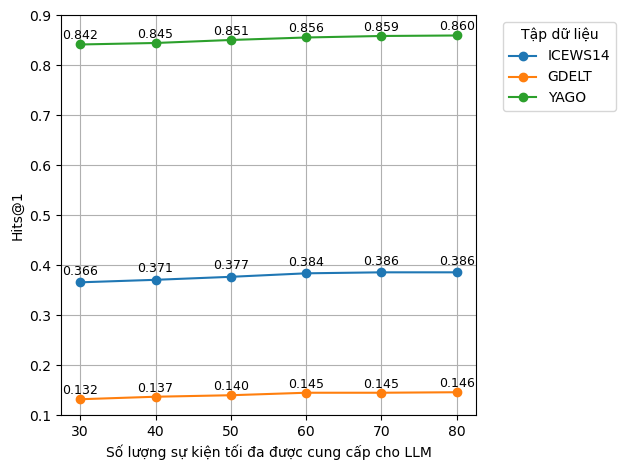
\includegraphics[width=0.8\textwidth]{images/max_number_retrieved_facts.png}
    \caption{Ảnh hưởng của số lượng sự kiện tối đa cung cấp cho LLM khi suy luận}
    \label{fig3: num_semantic_facts}
\end{figure}

Quan sát biểu đồ~\ref{fig3: num_semantic_facts}, ta thấy được chỉ số Hit@1 thể hiện xu hướng tăng lên sau đó
ổn định khi L tăng trên tập dữ liệu ICEWS14. Điều này cho thấy số lượng tối đa các sự kiện được cung cấp cho
LLM sẽ ảnh hưởng đến độ chính xác của nó. Trong trường hợp này, số lượng tối đa các sự kiện tốt nhất mà chúng ta nên cung cấp cho LLM là 60.